% !TeX spellcheck = en_US
\addscenariosection{1}{Clash Scenario}{The Fractured Kingdoms}{\images/two_way_monolith.png}

\begin{multicols}{2}

\textbf{Author:} mopo

\textit{A terrible Armageddon has stricken the lands. Five rulers have found their kingdoms broken and torn apart, but after some time has past, they found their lands have drifted in the magic-laden space of this universe to collide with 4 other kingdoms. All 5 recognize that their first priority must be to rebuild and regrow, and they make a 5-kingdom alliance. However, each also knows in the back of their minds that whoever would break the alliance first, would gain a sharp first-strike advantage...}

\subsection*{\MakeUppercase{Scenario Length}}
This Scenario is played over 16 Rounds.

\subsection*{\MakeUppercase{Player Setup}}
\textbf{Player Count:} 5 free-for-all

\textbf{Starting Resources:} 10 \svg{gold}, 6 \svg{building_materials}, 1 \svg{valuables}

\textbf{Starting Income:} 10 \svg{gold}, 0 \svg{building_materials}, 0 \svg{valuables}

\textbf{Starting Units:}
\begin{itemize}
  \item 3 × A Few \bronze\ Units
\end{itemize}

\textbf{Town Buildings:} \bronze\ Dwelling

\subsection*{\MakeUppercase{Map Setup}}
Take the following Map Tiles and arrange them as shown in the Scenario map layout:

\begin{itemize}
  \item 5 × Starting (I) Map Tile; \textbf{rotate them} so that their \textbf{blocked Fields} match the ones marked in the Scenario map layout
  \item 10 × Near (IV--V) Map Tile
  \item 10 × Far (II--III) Map Tile
  \item 5 × Center (VI--VII) Map Tile
\end{itemize}

\subsection*{\MakeUppercase{Victory Conditions}}
Score the most Victory Points (VPs) by the end of the \nth{16} Round.

\subsection*{\MakeUppercase{Timed Events}}

\textbf{\nth{4} Round:}
\begin{itemize}
  \item All yellow borders on the Starting (I) Map Tiles are ignored until the end of the game.
\end{itemize}

\subsection*{\MakeUppercase{Additional Rules}}
Before this Scenario:

\begin{itemize}
  \item Split the Artifact Deck by rarity into 3 separate Decks (Minor, Major, and Relic).
    A player may gain only Minor Artifacts on Starting or Far Tiles, Minor or Major Artifacts on Near Tiles, and Major or Relic Artifacts on Center Tiles.
  \item Split the Spell Deck into 2 separate Decks (Basic and Expert Spells). Magic Arrow is a Baiic Spell.
    A player may gain only Basic Spells on Starting or Far Tiles, Expert Spells on Near or Center Tiles.
\end{itemize}

During this Scenario:

\begin{itemize}
  \item Each \svg[12]{movement_token_green} in the map layout is a one-way portal.
    Any Hero on the Field an \svg[12]{movement_token_green} points away from can pay 1 \svgeven{movement} to go to the Field that \svg[12]{movement_token_green} is pointing to.
  \item You can defend your Town with your Hero if you have your Main Hero on your Starting (I) Map Tile.
  \item In addition to the regular tournament rules regarding scoring VPs, players gain VPs for the following:
  \item Owning the Grail Token increases your income by 5 \svg{gold}.
  \item In addition to the standard tournament rules regarding scoring VPs, players gain VPs for:
  \begin{itemize}
    \item 2 VP for flagging a Dragon Utopia
    \item 2 VP for having the Dragon Utopia flagged at the end of the game
  \end{itemize}
\end{itemize}

\subsection*{\MakeUppercase{Optional Rules}}
\begin{itemize}
  \item All \svg[12]{movement_token_green} indicate two-way portals instead of one-way.
    Heroes can travel in either direction by paying 1~\svgeven{movement}.
  \item The portals start inactive (place them the inactive \svg[12]{movement_token_red} side up).
    Heroes must pay 1~\svg{building_materials} and 1~\svgeven{movement} to activate them.
  \item Heroes can destroy portals by paying 1~\svgeven{movement}.
    Flip a destroyd portal the \svg[12]{movement_token_red} side up.
\end{itemize}

\end{multicols}

\vspace*{-6.5em}

\begin{tikzpicture}[overlay, remember picture]

  \newcommand{\blocked}[3]{%
    % Parameters: #1 = x-coordinate, #2 = y-coordinate, #3 = rotation angle
    \begin{scope}[shift={(#1,#2)}, rotate=#3]
      \draw[draw=darkyellow, thick, pattern=north east lines, pattern color=darkyellow]
        (0:0.56cm) -- (60:0.56cm) -- (120:0.56cm) --
        (180:0.56cm) -- (240:0.56cm) -- (300:0.56cm) -- cycle;
    \end{scope}
  }

  \newcommand{\arrow}[3]{
    % Parameters: #1 = x-coordinate, #2 = y-coordinate, #3 = rotation angle
    \node[rotate=#3, opacity=0.5] at ([shift={(2pt,-2pt)}]#1,#2) {
\includegraphics[height=23px]{\images/movement_token_shadow.png}};
    \node[rotate=#3] at (#1, #2) {\svg[20]{movement_token_green}};
  }

  \node(bg)[anchor=center, opacity=0.07, xshift=2em, yshift=-9em] at (current page.center) {
    
\includegraphics[width=1.25\paperwidth, keepaspectratio]{\art/two_way_monolith.png}
  };

  \node at (9, -12) {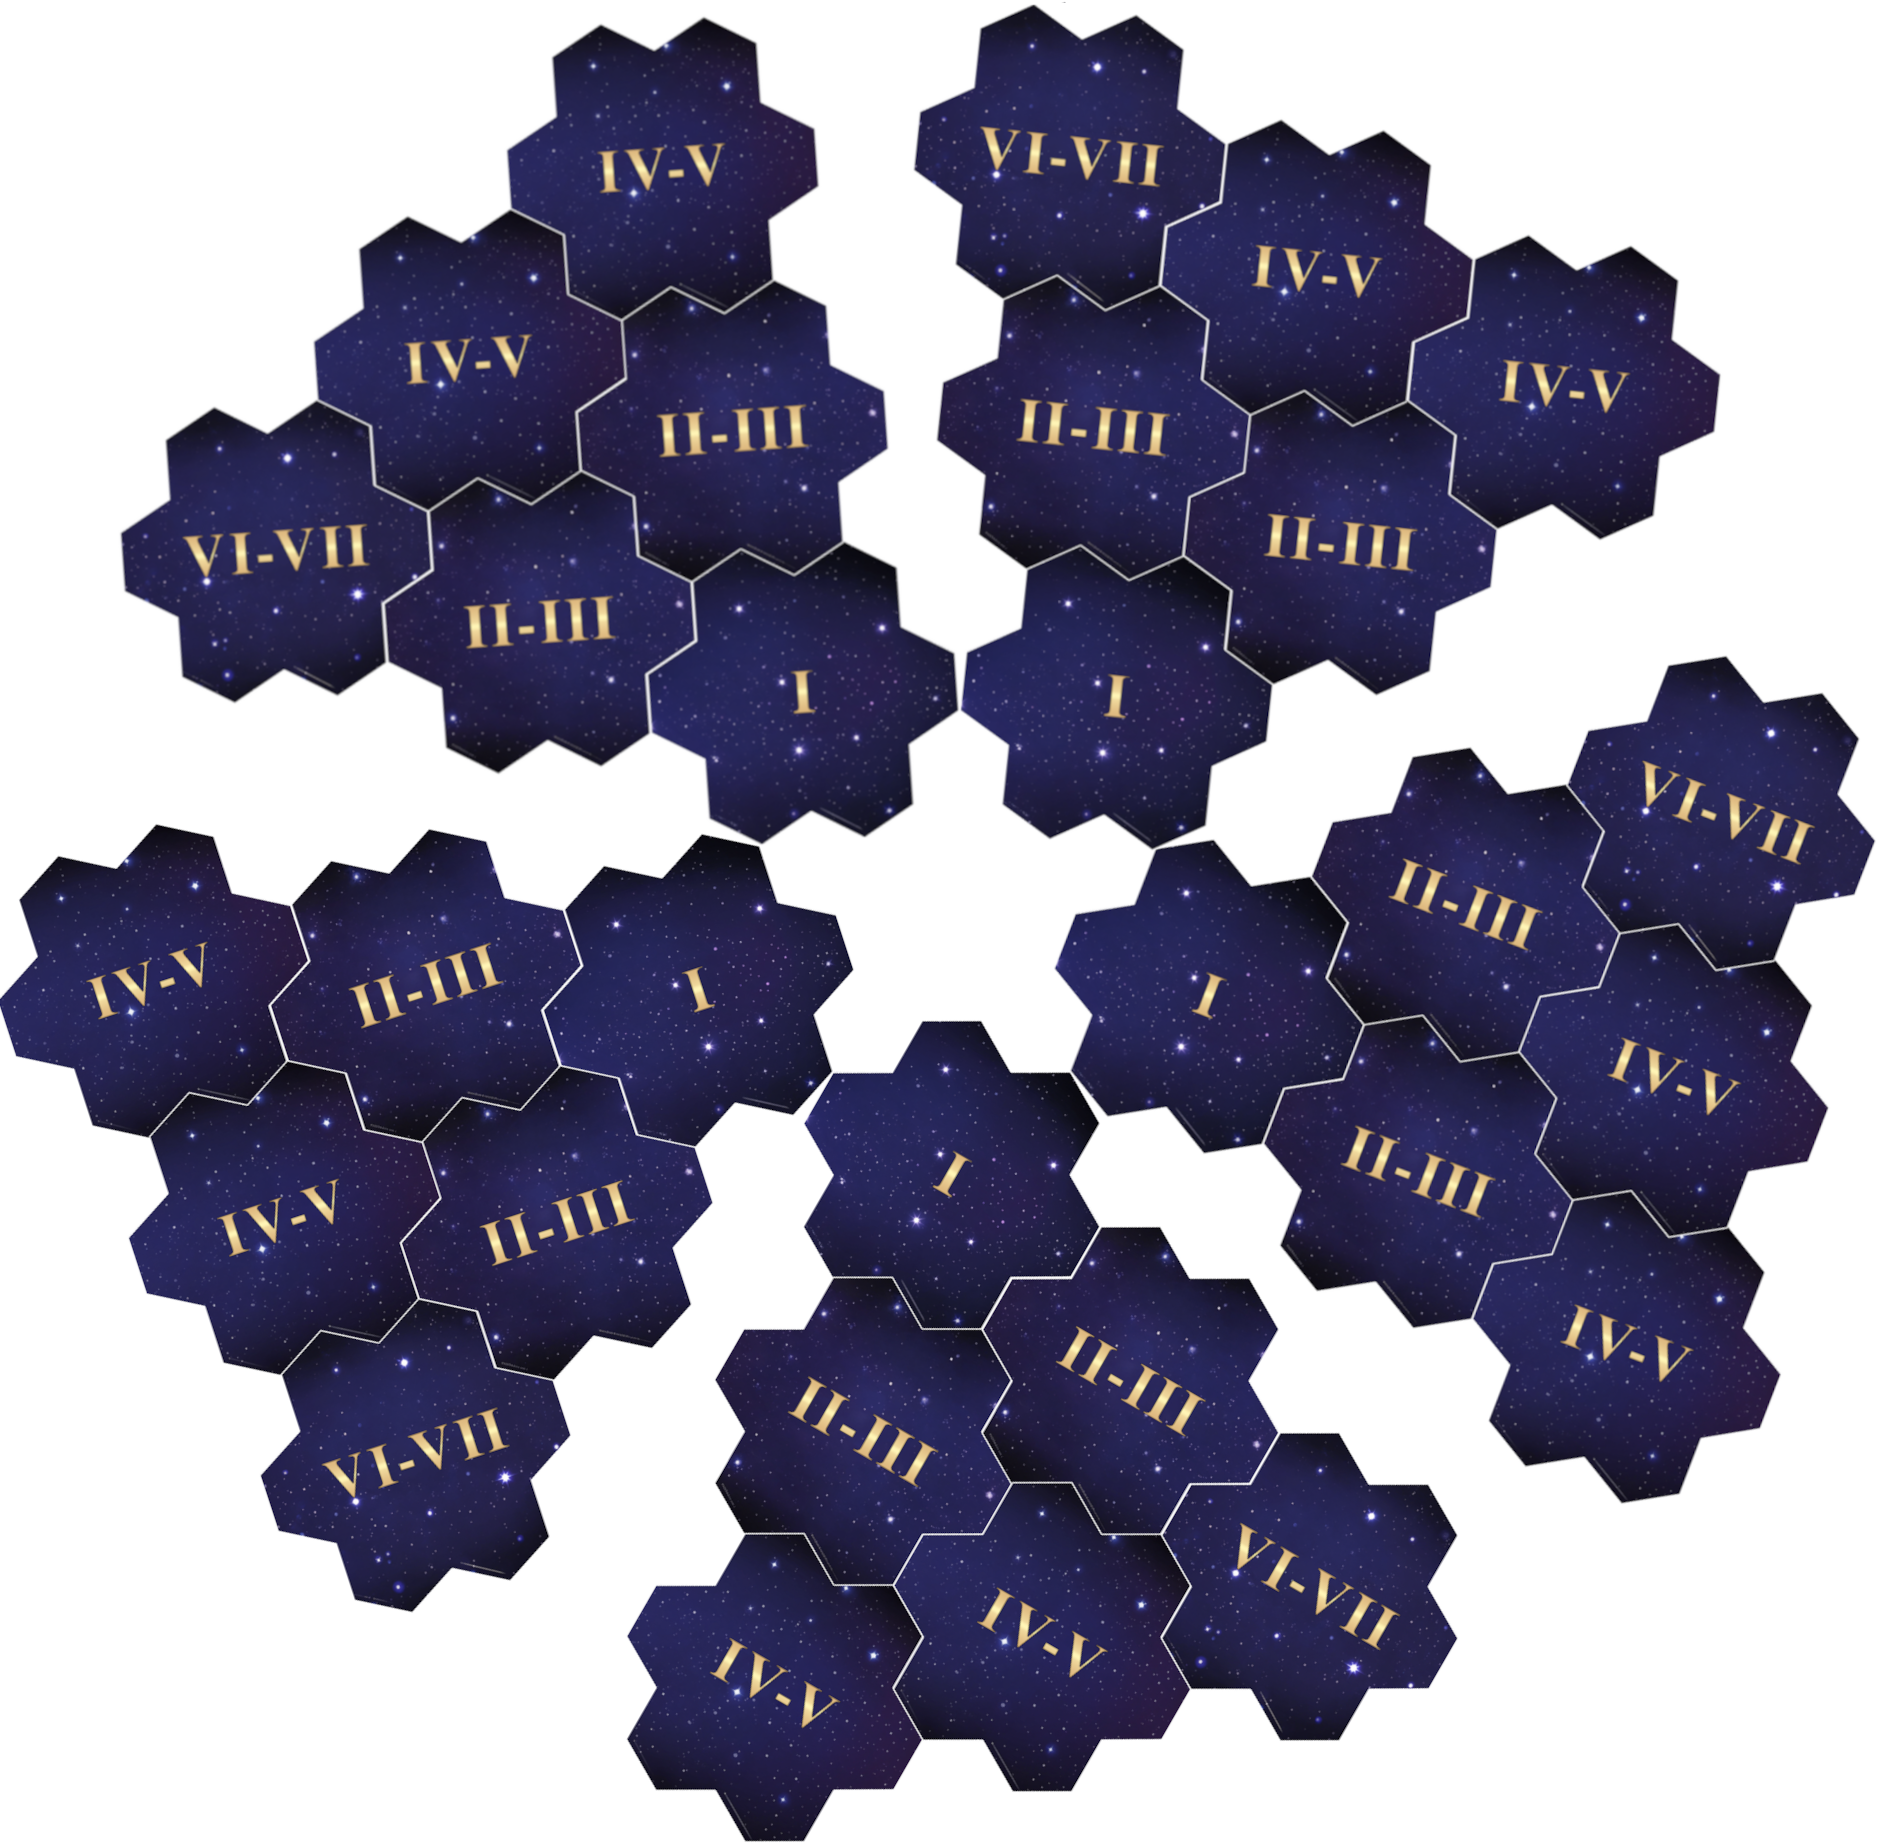
\includegraphics[width=0.9\paperwidth]{\maps/the_fractured_kingdoms.png}};

  \arrow{12.35}{-15.7}{-142}
  \arrow{14.4}{-17.6}{38}

  \arrow{13.91}{-9.95}{-72}
  \arrow{16.2}{-8.55}{108}

  \arrow{8.2}{-4.35}{-176}
  \arrow{8.75}{-6.9}{4}

  \arrow{1.5}{-10.35}{-99}
  \arrow{4.2}{-10.75}{81}

  \arrow{6.65}{-16.1}{155}
  \arrow{5.45}{-18.7}{-25}

  \blocked{7.05}{-8.85}{-25.5}

  \blocked{11.40}{-8.87}{23}

  \blocked{12.69}{-13.12}{67.7}

  \blocked{9.135}{-15.58}{0}

  \blocked{5.58}{-13.01}{-71}


\end{tikzpicture}
